% uncomment this for line numbering;
% Note: \usepackage{lineno} does NOT work with revtex!
\RequirePackage{lineno}
\documentclass[aps,prb,preprint,groupedaddress,showkeys]{revtex4}
\usepackage[pdftex]{graphicx}
\usepackage[colorlinks=true,linkcolor=blue,citecolor=blue]{hyperref}
%\usepackage{lineno}
% declare the path(s) where your graphic files are
% and their extensions so you won't have to specify these with
% every instance of \includegraphics

%%%% uncomment this for Techincal Notes:
%\setcounter{secnumdepth}{0}
\usepackage{booktabs, multirow}
\usepackage{siunitx}
\usepackage{gensymb}
\usepackage{subfigure}
\usepackage{dcolumn}% Align table columns on the decimal point

\usepackage{url}


\begin{document}

\def\papertitle{Two-stage deep learning framework for the restoration of incomplete-ring PET images}
\title{\papertitle}

\author{Yeqi~Fang}
\email[Email: ]{fangyeqi@stu.scu.edu.cn}
\affiliation{College of Physics, Sichuan University, Chengdu, 610065, China}
\author{Rong~Zhou}
\affiliation{College of Physics, Sichuan University, Chengdu, 610065, China}

\date{\today}

\begin{abstract}
\textbf{Purpose:} Positron Emission Tomography (PET) is an important molecular imaging tool widely used in medicine. Traditional PET systems rely on complete detector rings for full angular coverage and reliable data collection. However, incomplete-ring PET scanners have emerged due to hardware failures, cost constraints, or specific clinical needs. Standard reconstruction algorithms often suffer from performance degradation with these systems because of reduced data completeness and geometric inconsistencies.

\textbf{Methods:} We present a two-stage deep-learning framework that, without incorporating any time-of-flight (TOF) information, restores high-quality images from data with about 50\% missing coincidences—double the loss levels previously addressed by CNN-based methods. The pipeline operates in two stages: a projection-domain Attention U-Net first predicts the missing sections of the sinogram by leveraging spatial context from neighbouring slices, after which the completed data are reconstructed with OSEM algorithm and passed to a U-Net–diffusion module that removes residual artefacts while reinstating high-frequency detail.

\textbf{Results:} Using 206 brain volumes from a public dataset, the result shows that our model successfully preserves most anatomical structures and tracer distribution features with PSNR of 35.92 dB and SSIM of 0.9958.

\textbf{Conclusion:} our two-stage deep‐learning framework effectively restores high‐quality PET images from over 50 \% incomplete‐ring data, achieving near‐complete anatomical fidelity and robust performance without requiring TOF information.
\end{abstract}

\keywords{Incomplete‐ring, Sinogram restoration, Attention U‐Net, Diffusion‐based refinement}
\maketitle

% \linenumbers\modulolinenumbers[5]

\section{Introduction}
\label{chap:introduction}

Positron emission tomography (PET) is a powerful molecular imaging technique that provides quantitative visualization of metabolic processes within living tissue \cite{townsend2004, muehllehner2006positron, lameka2016positron, shukla2006positron, nutt2002history}. PET operates on the principle that positrons annihilate upon encountering electrons, producing detectable 511keV photon pairs: a radiotracer introduces positrons that annihilate upon encountering electrons, and then produce pairs of $511$keV photons traveling in opposing directions. 
The photon pairs are then detected by a pair of scintillation sensors, and each coincidence event will define a line-of-response (LOR).
Traditional PET systems usually use complete 360$^\circ$ detector rings to maximize their sensitivity and angular coverage \cite{townsend2004}.

However, incomplete-ring systems have emerged from practical necessity rather than theoretical preference: they reduce costs and complexity, allow closer access to patients in specialized applications like breast scanning or in-beam therapy monitoring \cite{surti2008}, create "open" configurations that alleviate claustrophobia \cite{tashima2012, krishnamoorthy2021}, and enable novel applications such as dual-panel brain imaging systems \cite{zhang2020}. The trade-off is severe—incomplete angular coverage creates gaps in projection data, turning reconstruction into an underdetermined problem. Missing angular views inevitably introduce artifacts and resolution non-uniformity \cite{kak1988, surti2008}. Even time-of-flight capabilities, which partially fix these problems, can't fully compensate for limited view angles \cite{surti2008, krishnamoorthy2021}.

Researchers have investigated a lot of methods to achieve better and better incomplete-ring PET reconstruction. Analytical ways like filtered back-projection falter immediately—their assumption of complete data leads to pronounced streak artifacts \cite{kak1988}. Iterative approaches like maximum-likelihood expectation-maximization (MLEM) are better by modeling the acquisition process \cite{qi2006}, but they still have artifacts along missing view directions \cite{zhang2020}.
Penalized likelihood methods incorporating prior constraints show promise, as Zhang \textit{et al.} demonstrated by using high-quality prior images to enhance contrast recovery in a dual-panel head-and-neck PET system \cite{zhang2020}. And sinogram completion approaches attempt to estimate or interpolate the absent projection data prior to reconstruction \cite{makkar2024partial}. But these methods are still not enough to solve the fundamental problem. 

Deep learning has shown remarkable success in many fields \cite{PhysRevD.110.063011, liu2024deep, reader2020deep}. Regression-based networks have shown promise in low-dose PET denoising and partial data reconstruction \cite{Kandarpa_2021} by learning direct mappings between degraded and high-quality images. Liu \textit{et al.}'s U-Net approach to transform artifact-degraded partial-ring PET images \cite{liu2019} demonstrated initial success, but the model in this work is mainly targeted for mild data loss and training data didn't consider the context of sinograms.
However, current available techniques have some drawbacks.
For examples, while GAN approaches are good at generating visually compelling reconstructions, \cite{xue2023cg3dsrganclassificationguided3d} they are unstable when training and often highly sensitive to hyperparameters, which limit their clinical use.
Methods based on explicit likelihood modeling—like VAEs and flow-based approaches—offer solid theoretical foundations. But they usually lose details in reconstructed images and their low speeds also make them not suitable for clinical use.
Model-based deep learning frameworks and generative models \cite{reader2023, vashistha2024} show promise but risk introducing hallucinated features—a dangerous proposition in medical imaging.

In this work we introduce a two-stage deep-learning framework that restores highly degraded partial-ring PET data and, for the first time, is validated under $>$ 50 \% coincidence loss.  Our contributions are four-fold: 
(1) we propose a five-channel slice-stacking strategy that fuses immediate spatial and axial neighbours in the sinogram, providing rich local context for projection restoration; 
(2) missing‐angle gaps are reconstructed with an Attention U-Net specifically tuned for severe angular deficits, enabling the network to focus selectively on informative sinogram regions; 
(3) the resulting OSEM images are passed to a lightweight residual-diffusion module that iteratively synthesises high-frequency details while suppressing artefacts, thereby decoupling data completion from perceptual refinement; 
and (4) we establish the first systematic benchmark on 206 public brain volumes with half the coincidences removed, demonstrating that our pipeline achieves 35.92 dB / 0.9958 SSIM in image space and runs in $<$ 2 s per image on a single GPU—surpassing existing partial-ring methods without hand-tuned regularisation.

The remainder of this thesis is organized as follows:
\textbf{Section~\ref{chap:background}} provides an overview of PET and its basic physics like principles of coincidence detection, and the main problems caused by incomplete rings. We also summarize classical and modern reconstruction methods.
\textbf{Section~\ref{chap:methods}} presents our contribution in full: the simulation framework for complete and partial rings, the projection-completion Attention U-Net, the subsequent OSEM reconstruction, and the diffusion-based image-refinement module, together with implementation and training details.
\textbf{Section~\ref{chap:results}} reports quantitative and qualitative evaluations on 206 brain volumes under several angular-loss patterns, comparing sinogram restoration, preliminary OSEM images and final refined outputs.
\textbf{Section~\ref{chap:conclusion}} summarizes our findings by analysing metrics of model performance on test dataset, and discusses limitations and directions for future improvements.
\textbf{Appendices} provide additional experiments, extended qualitative results, and tables of hyperparameters used in the study.




\section{System Model and Data Simulation}

\label{chap:background}




\begin{figure*}[htbp]
    \centering
    \vspace{-0.2cm}
    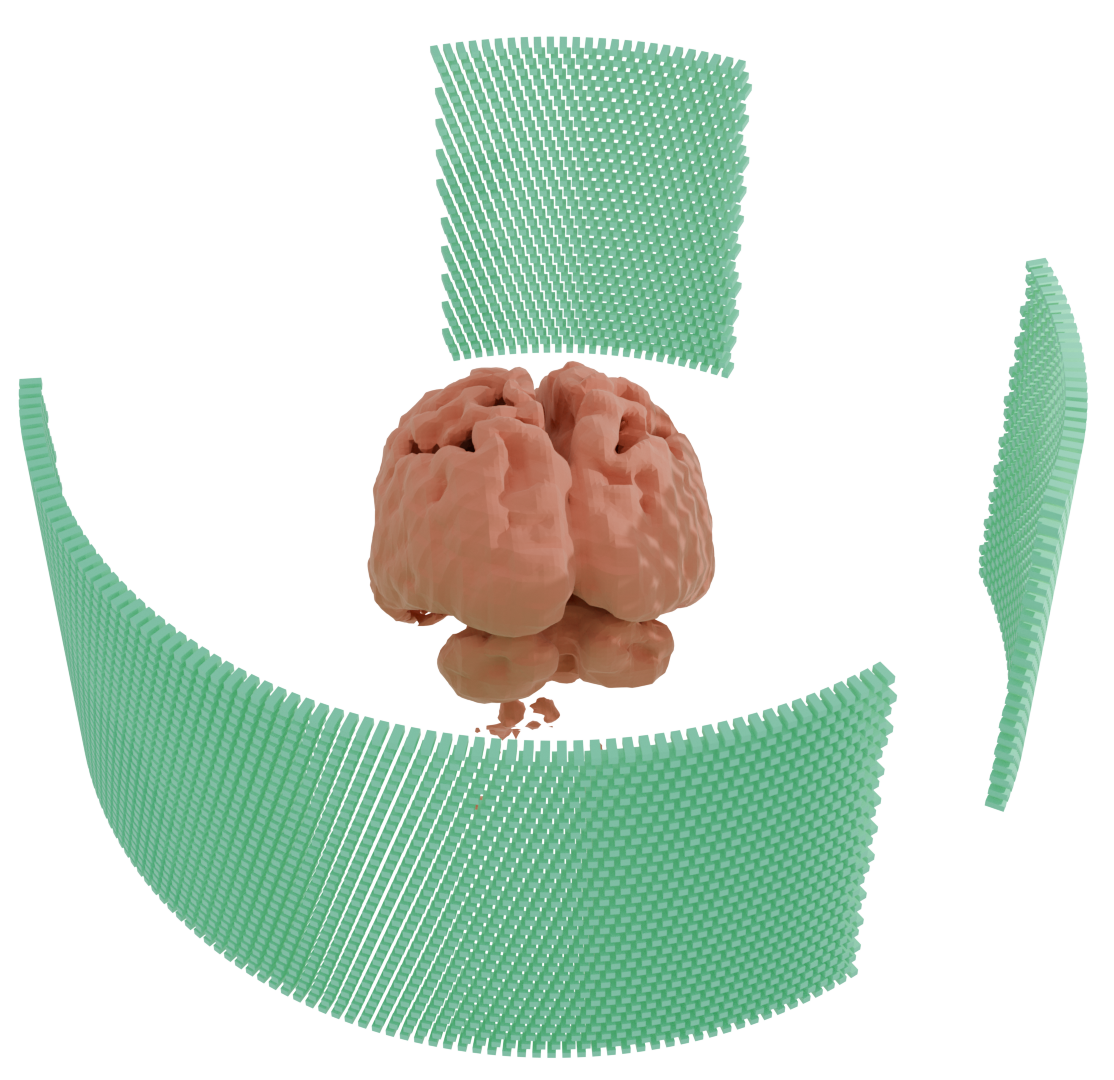
\includegraphics[width=0.34\textwidth]{Images/Thehumanbrainismissing5}
    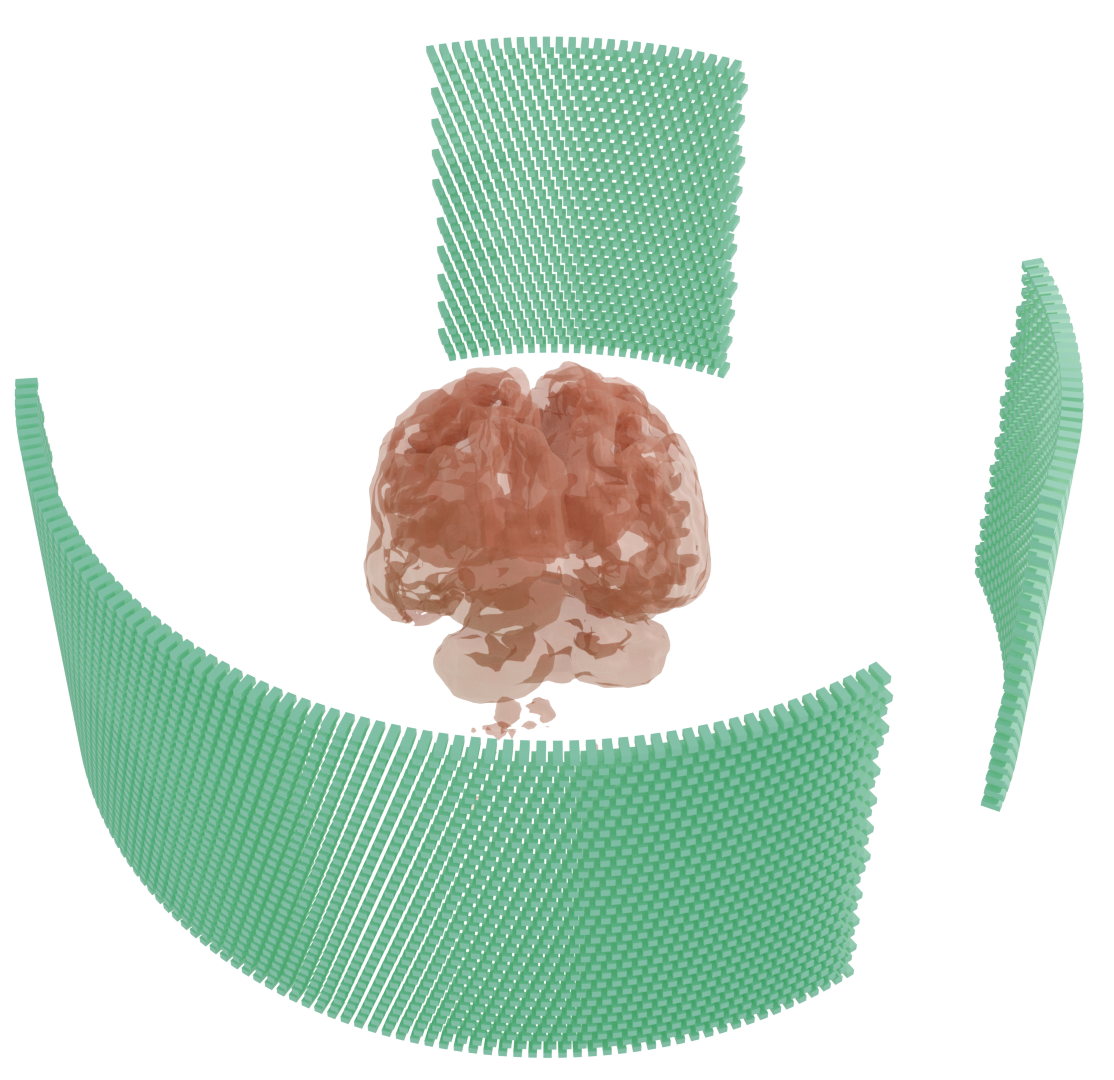
\includegraphics[width=0.34\textwidth]{Images/Thehumanbrainismissing4}
    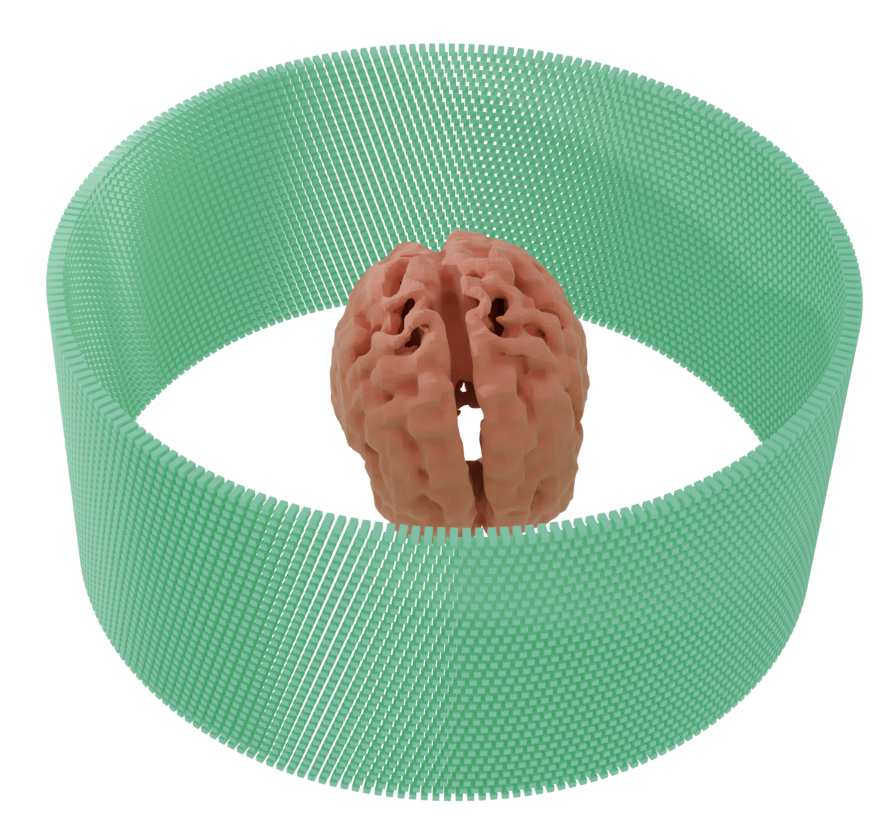
\includegraphics[width=0.34\textwidth]{Images/Thehumanbrainisnotmissing3}
    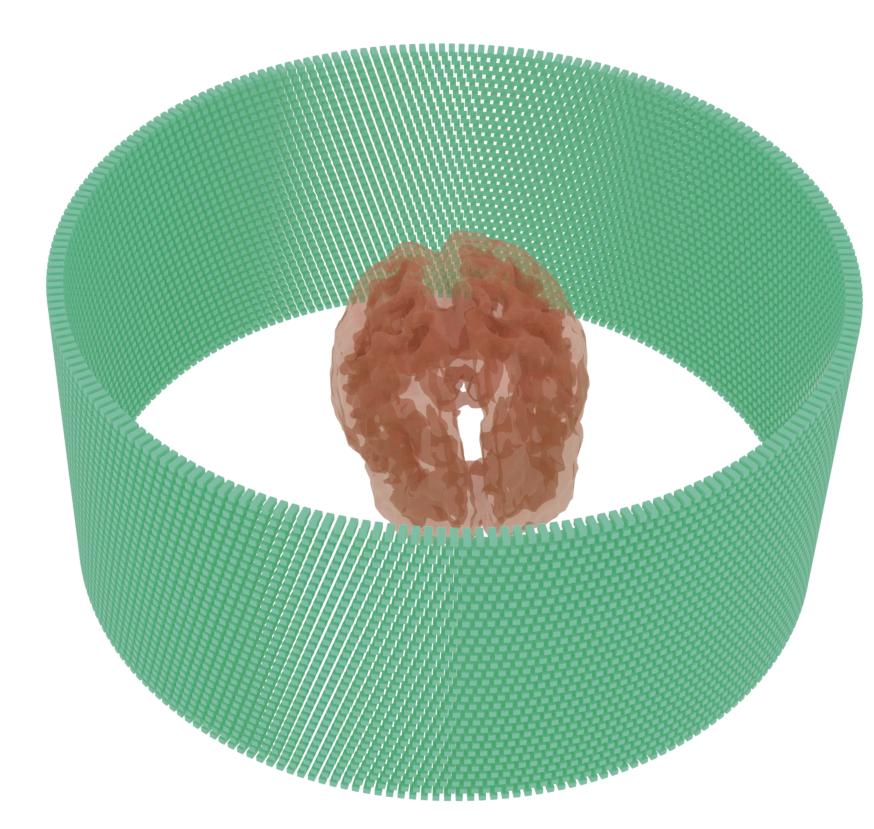
\includegraphics[width=0.34\textwidth]{Images/Thehumanbrainisnotmissing4}
    \vspace{-0.2cm}
    \caption{Three-dimensional schematic of incomplete and complete ring PET scanner detector structure, with the right image showing a perspective view.}
    \vspace{-0.2cm}
    \label{fig:pet_structures2}
\end{figure*}

% When two detectors measure gamma photons within a narrow time window (typically 6-12 nanoseconds), we assume they are from the same annihilation event. This paired detection forms a line of response (LOR) between the two detectors.
% PET systems record these events in one of two primary formats. In \textbf{list-mode data}, each coincidence is logged individually with precise identification of the detector pair and timestamp. This approach saves the maximum amount of information but generates enormous datasets. \textbf{Sinogram data} organizes coincidence events into radial, angular, and axial bins, creating a structured histogram that trades off temporal resolution for simpler processing. Standard PET scanners use 360$^\circ$ detector rings to achieve uniform LOR sampling, but things would be quite different when this ideal geometry isn't possible.






Incomplete ring configurations arise from practical constraints including cost limitations, hardware failures, and specific clinical requirements. Budget constraints often drive this compromise—each detector module constitutes a substantial cost, and reducing their number can make PET technology accessible to more facilities. In specialized applications, partial ring designs actually provide benefits: breast imaging benefits from closer detector positioning, interventional procedures require open scanner designs, and claustrophobic patients experience less anxiety with more open configurations.





The consequences of missing detectors are profound. 
LORs that would normally pass through the missing sections simply vanish from the dataset, creating angular sampling gaps. The results collapse under data deficiency if we directly reconstruct the image out of incomplete sinogram, as shown in Figure~\ref{fig:pet_incomplete_reconstruction}.

% \subsection{System Model and Data Simulation}

To deal with these problems systematically, we made a thorough simulation framework modeling both complete and incomplete PET geometries. Our approach begins with a standard ring configuration of $R$ axial rings (we used $R=42$ in our experiments), each containing $D=182$ detectors arranged cylindrically. The scanner radius ($\rho$) of 253.71 mm balances spatial resolution against sensitivity.

% Early in our research, we attempted to use Transformer-based approaches for direct 3D image recovery, following Hatamizadeh et al.'s UNETR framework \cite{hatamizadeh2021unetrtransformers3dmedical}. The segmentation results were excellent, but when applied to our incomplete sinogram data, these methods did not work well, with SSIM of less than 0.2 even after a long time of training. This indicates that mere geometric information is insufficient for high-quality reconstruction when some angular segments are missing. 



From listmode to sinogram, and from sinogram to reconstruction, the information is constantly losing. So, rather than attempting direct image-domain recovery, we pivoted to a two-stage method—first converting listmode data to sinograms with missing sections, then applying specialized techniques to complete these sinograms before final reconstruction. This approach, while computationally more intensive, provided a more applicable way to solve the missing data problem by retaining as much information as possible from sinogram.
For simulation purposes, we mapped a $128\times128\times128$ voxel grid to physical space, yielding in-plane voxel dimensions of approximately 2.78 mm.


\begin{figure*}[htbp]
    \centering
    \vspace{-0.2cm}
    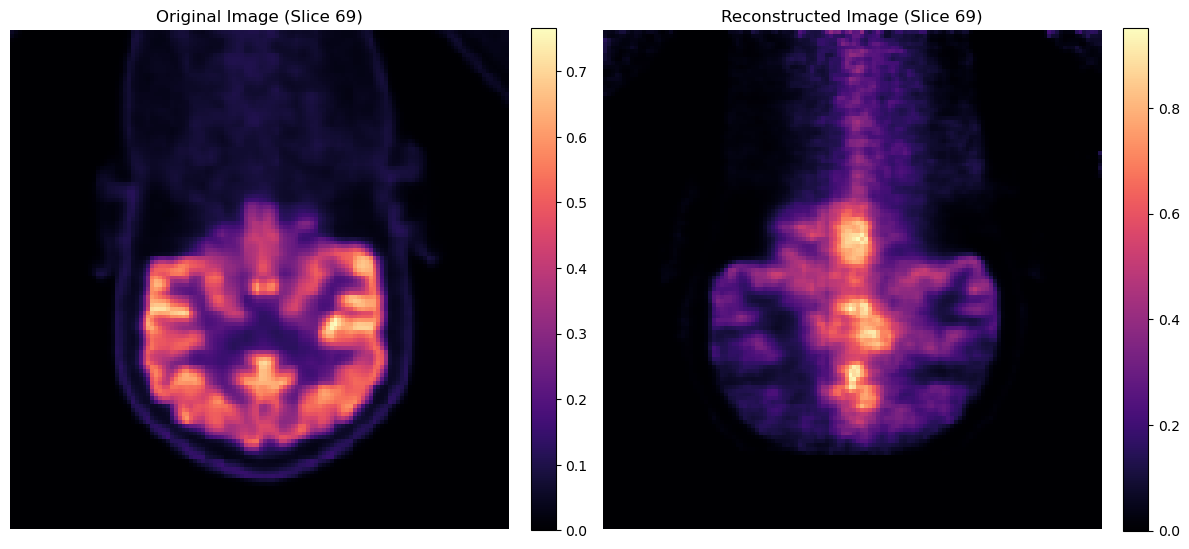
\includegraphics[width=0.8\textwidth]{Images/output2}
    \vspace{-0.2cm}
    \caption{Comparison of reconstruction results from incomplete rings with the original image, showing that the two are vastly different, demonstrating that direct reconstruction from incomplete rings is not feasible.}
    \vspace{-0.2cm}
    \label{fig:pet_incomplete_reconstruction}
\end{figure*}

The detector system configuration is based on our planned experimental setup for future validation studies. Table \ref{tab:detector_params} describes the specific configuration parameters of our target PET system, which represents the specifications of an incomplete-ring PET scanner currently under development in our laboratory. 
Our PET system simulation employed the Monte Carlo simulation toolkit SimSET (Simulation System for Emission Tomography) \cite{Harrison157P} to model a realistic full-ring PET scanner geometry (Siemens Biograph mMR) \cite{Delso1914}. The scanner consists of 56 detector blocks per ring and 8 blocks along the scanner axis, with each detector block containing $8 \times 8$ lutetium oxyorthosilicate (LSO) crystals ($4 \times 4 \times 20$mm). The energy resolution was set to 14.5\% full-width-at-half-maximum at 511keV.

\begin{table}[htbp]
    \centering
    \caption{PET Scanner Configuration Parameters (based on our planned experimental prototype for future validation studies)}
    \label{tab:detector_params}
    \begin{tabular}{l l}
    \hline \hline \addlinespace[2pt]
    \textbf{Parameter} & \textbf{Value} \\
    \hline\addlinespace[2pt]
    Radius & 253.71 mm \\
    Crystal transaxial spacing & 4.02 mm \\
    Crystal axial spacing & 5.37 mm \\
    Module axial spacing & 37.56 mm \\
    Crystal elements (transaxial) & 13 \\
    Crystal elements (axial) & 7 \\
    Transaxial sectors & 28 \\
    Axial sectors & 1 \\
    Modules (axial) & 6 \\
    Crystals per ring & 182 \\
    Number of rings & 42 \\
    \hline \hline
    \end{tabular}
\end{table}

% Our theoretical model parameters is an idealized PET system, setting aside real-world manufacturing variations that would typically require complex normalization procedures. 
% While our framework includes parameters for TOF detection, we chose not to implement this capability in the current work, because the devices to which we intend to apply this study do not have that high temporal resolution. 
% Similarly, our simulation framework does not account for attenuation correction problems needing MRI or CT data in physical implementations—an important consideration for future translation of our approach. 

% Our simulation generates idealized datasets by ray-tracing approximately 20 million emission events from $80\times128\times128$-voxel phantom images, creating perfectly clean list-mode data without the noise and artifacts present in real-world situation. 
% We used a dataset of 206 brain PET volumes, each with dimensions of $128^3$-voxel from a public dataset as phantom images for our simulation \cite{Han2023DiffusionPET}. Each image simulates 2 billion events, the detectors detect 560 million events on average and record them in the listmode data. We then removed detectors with angles between [30\degree, 90\degree] and [210\degree, 270\degree]. This meant that any LOR with either detector within these two angular ranges cannot be recorded. Incomplete sinograms generated in this configuration only have about 306 million events, accounting for 54.6\% of the originally detected events.



A 15-minute static FDG brain PET scan was simulated, equivalent to an average of 280 million coincidence events including both true and scatter events. The activity ratio of gray matter (GM) to white matter (WM) was set to 4:1, while the rest of the brain tissue was assumed to have no activity uptake. Importantly, the attenuation effects of seven tissue types (connective tissue, water, brain, bone, muscle, fat, and blood) were incorporated in the simulations and subsequently corrected during image reconstruction, providing a more realistic modeling of clinical PET acquisitions.

We used a dataset of 206 brain PET volumes from 206 individual healthy human subjects, each with dimensions of $128^3$ voxels from a public dataset as phantom images for our simulation \cite{Han2023DiffusionPET}. All subjects had normal brain anatomy without any pathological conditions, ensuring consistent baseline characteristics across the dataset. The dataset exhibits natural anatomical variation typical of healthy adult brains, including differences in brain size, cortical folding patterns, and regional tissue distributions. Each phantom was down-sampled to a matrix of $128 \times 128 \times 128$ with voxel size of $2.78 \times 2.78 \times 2.78$mm$^3$. This healthy brain dataset provides a robust foundation for evaluating our reconstruction framework's performance on normal anatomical structures before extending to pathological cases in future studies.

The complete ring configuration (Figure~\ref{fig:pet_structures2}) provides our reference reconstruction $\mathbf{Y}_A$, representing the best-case scenario with full angular sampling. For incomplete ring experiments, we selectively remove detectors—either entire rings or angular segments—and generate a degraded reconstruction $\mathbf{Y}_B$ from the resulting partial data. The striking quality difference between $\mathbf{Y}_A$ and $\mathbf{Y}_B$ shows the reconstruction challenge we aim to solve, as shown in Figure~\ref{fig:pet_incomplete_reconstruction}.

% \subsection{Conventional PET Reconstruction Methods}

% Before introducing new solutions, Several popular reconstruction approaches that are not based on machine learning have been assessed.
% Currently, main powerful methods are \textbf{maximum likelihood methods}, particularly MLEM and its faster variant OSEM \cite{363108}, which include the Poisson statistics of photon counting. The most important parameter of these two approaches is \textbf{system model}, which relates image voxels to measured projections:
% \begin{equation}
%     y_i \;\approx\; \sum_{j} p_{ij}\,\lambda_j,
% \end{equation}
% Here, $\lambda_j$ is the activity in voxel $j$, $y_i$ is the count measured in projection $i$, and $p_{ij}$ is the probability that an emission from voxel $j$ is detected along projection $i$. This \textbf{system matrix} $p_{ij}$ includes all the physics—from detector geometry to attenuation effects—that connects the unknown tracer distribution to our measurements.

% MLEM iteratively updates the estimate of $\lambda_j$ according to:
% \begin{equation}
%     \lambda_j^{(k+1)}
%     \;=\;
%     \lambda_j^{(k)}
%     \;\times\;
%     \frac{\displaystyle \sum_{i=1}^{N} \frac{p_{ij}}{\sum_{\ell} p_{i\ell}\,\lambda_{\ell}^{(k)}} \; y_i}
%     {\displaystyle \sum_{i=1}^{N} p_{ij}}.
% \end{equation}
% However, MLEM's convergence is too slow for large datasets. OSEM makes this process faster by dividing projections into subsets and then update the image estimate using one subset at a time:
% \begin{equation}
%     \lambda_j^{(k+1)}
% \;=\;
% \lambda_j^{(k)}
% \;\times\;
% \frac{\displaystyle \sum_{i \in S_{k}} \frac{p_{ij}}{\sum_{\ell} p_{i\ell}\,\lambda_{\ell}^{(k)}} \; y_i}
% {\displaystyle \sum_{i \in S_{k}} p_{ij}}
% \end{equation}
\begin{figure*}[ht]
    \centering
    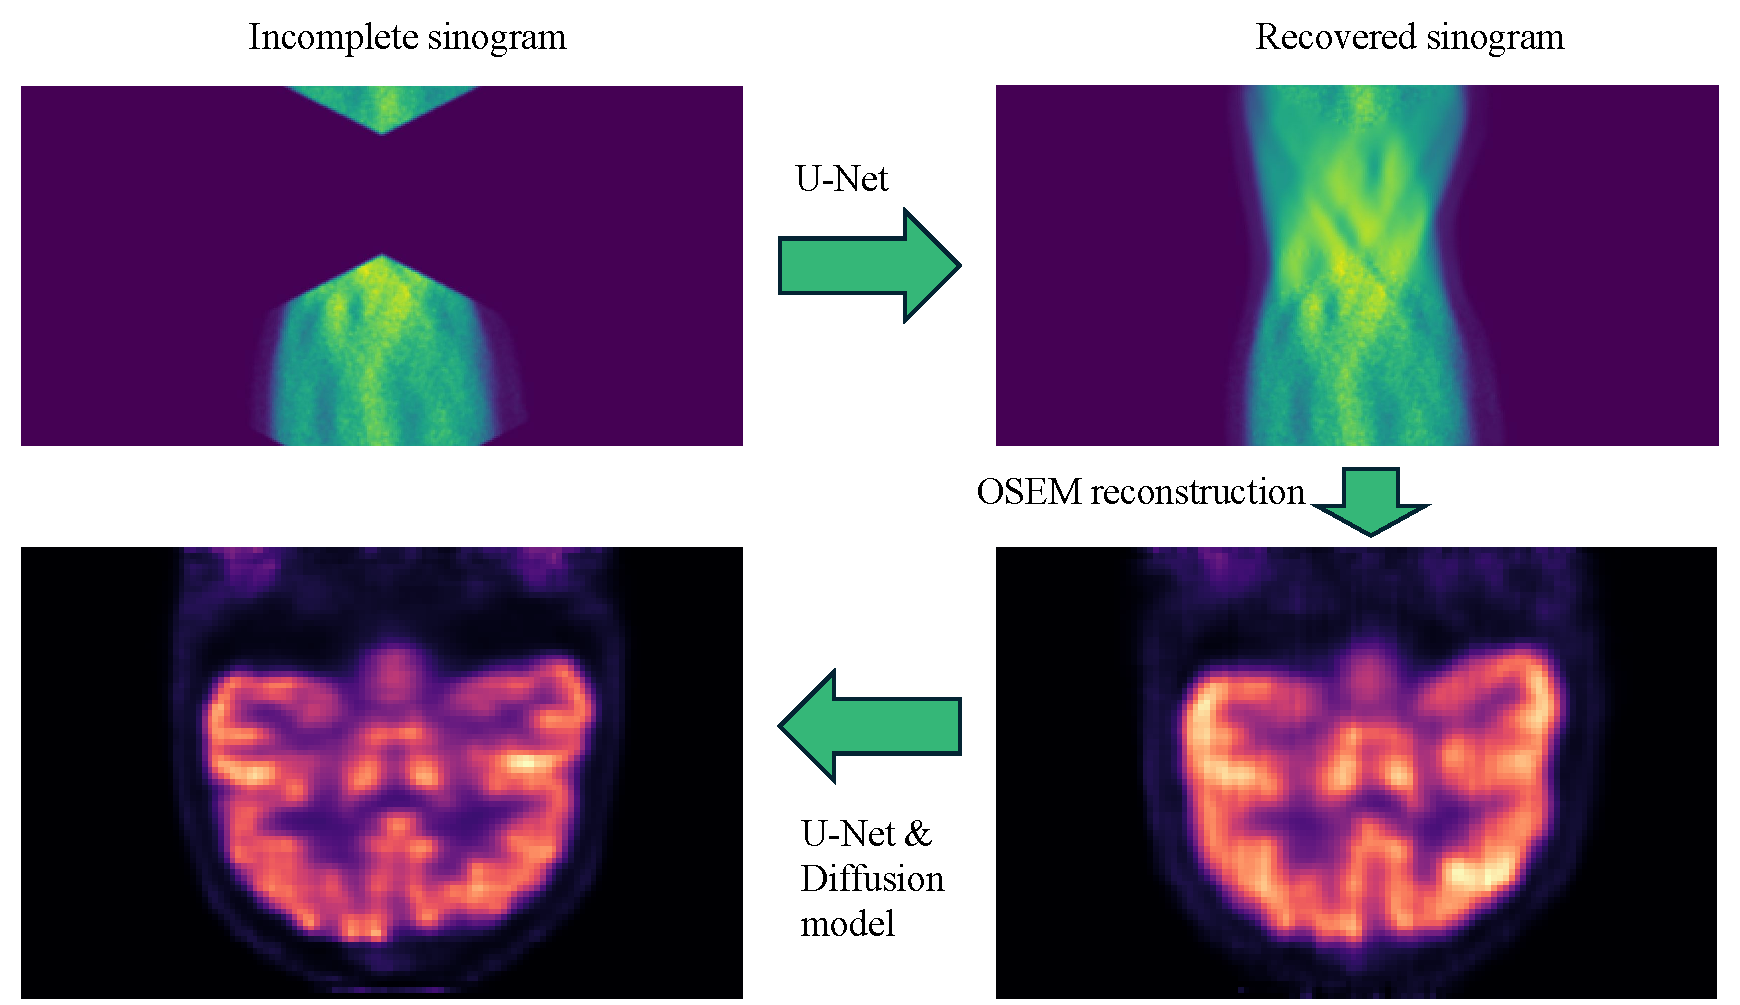
\includegraphics[width=\textwidth]{Images/reconstruction_workflow}
    \vspace{-.5cm}
    \caption{Overall flow diagram of the incomplete ring PET reconstruction method. First, incomplete sinograms due to missing detectors are repaired through a U-Net deep learning model to generate complete sinogram data . Then the complete sinogram is converted into a PET image using the OSEM iterative reconstruction algorithm.  finally, the image is refined using a U-Net \& diffusion model to remove residual artifacts and enhance high-frequency details. 
  }
    \vspace{-.2cm}
    \label{fig:reconstruction_workflow}
\end{figure*}
% Our work mainly depend on the PyTomography library \cite{POLSON2025102020}, which make use of PyTorch and GPUs to make intense computations a lot faster. This technique is important when reconstructing large listmode data with around one billion events.
% While OSEM is powerful with full angular sampling, its performance with incomplete rings was disappointing [cf.~Figure~\ref{fig:pet_incomplete_reconstruction}]. Because the missing angles also mean information loss that makes any iterative methods impossible to recover, despite their statistical sophistication. 
% Thus, OSEM can only be useful if the sinogram is complete or recover to a complete one. But it can not solve the core problem of missing data.




\section{Methods}
\label{chap:methods}


As shown in Figure \ref{fig:reconstruction_workflow}, this study proposes an innovative incomplete ring PET reconstruction framework that effectively addresses the data incompleteness problem caused by missing detectors through a multi-stage strategy. In the first stage, the system first processes incomplete sinograms (top left) resulting from missing detectors, completing the missing data through a trained optimized U-Net deep learning model to generate complete sinograms (top right). This sinogram restoration process fully utilizes the five-channel input strategy, effectively integrating spatial and temporal context information.


\subsection{Sinogram Reconstruction Based on Attention U-Net}
\label{sec:unet_sinogram}

Sinogram repair is fundamental in incomplete ring PET imaging, as its quality directly affects the precision of reconstructed images. 
The shape of sinogram tensors is $(D, 2D+1, R^2)$, or $(182, 365, 1764)$ in our work, where $R$ is the number of axial rings and $D$ is the number of detectors each ring. And it is obvious that this tensor is too large to be directly fed into any UNet-like models. So we cut this large $(D, 2D+1, R^2)$ tensor into $R\times(D, 2D+1, R)$ tensors. 
As shown in Figure~\ref{fig:sinogram_structure}, the central channel of each input tensor corresponds to the current sinogram slice, while the direct spatial neighbors (slices $j-1$ and $j+1$) and temporal neighbors from previous and subsequent sinogram periods (slices $j-R$ and $j+R$) constitute the other four channels. For boundary handling, when adjacent indices exceed the dataset range, the central slice itself is used for channel filling, ensuring input dimension consistency. These neighboring slices are important for improving the model's understanding of local structural continuity and temporal consistency. So finally we have $1764\times(182, 365, 5)$ tensors for each sinogram. 
To make sure each image was evaluated once in the test set, we implemented 6-fold cross-validation across the 206 volumes (4 groups with 34 images and 2 groups with 35 images). The predictions obtained from our model were reconstructed using the OSEM algorithm to achieve preliminary geometric recovery, and these reconstructions were subsequently used as inputs for our second stage framework.

Although traditional U-Net performs excellently in medical image segmentation and reconstruction tasks \cite{ronneberger2015unetconvolutionalnetworksbiomedical}, it lacks the ability to selectively focus on key features when dealing with complex incomplete ring PET sinogram restoration problems. The Attention U-Net \cite{oktay2018attentionunetlearninglook} adopted in this study enhances the model's perception of important feature regions through spatial attention mechanisms while suppressing the influence of irrelevant features, which is more useful for restoring sinograms from incomplete data. We also tested some transformer-based U-Net like UNETR \cite{hatamizadeh2021unetrtransformers3dmedical}, which combines ViT encoder and convolutional decoder, and TransUNet \cite{chen2021transunettransformersmakestrong}, where both encoder and decoder are completely based on transformers. But they are slightly outperformed by Attention U-Net.

The main innovation of Attention U-Net is the introduction of attention gating (AG) modules in the skip connection path of the original U-Net. These AG modules can adaptively highlight significant structures in the feed-forward feature maps while suppressing less relevant regions. 
For sinogram reconstruction tasks, this mechanism is especially useful as it can selectively focus on structural features around missing areas, and then more accurately infer missing angular data. The mathematical expression of attention gating can be described as \cite{oktay2018attentionunetlearninglook}:
\begin{equation}
\alpha_i^l = \sigma_2(\psi^T(\sigma_1(W_x^T x_i^l + W_g^T g_i + b_g)) + b_\psi),
\end{equation}
where $x_i^l$ is the low-level feature from the encoder, $g_i$ is the gating signal from the decoder (high-level feature), $\sigma_1$ and $\sigma_2$ are ReLU and Sigmoid activation functions respectively, and $W_x$, $W_g$, $b_g$, and $b_\psi$ are learnable parameters. $\alpha_i^l \in [0,1]$ is the calculated attention coefficient used to control the importance of features.
After processing through the attention gate, the features can be represented as:
\begin{equation}
\hat{x}_i^l = x_i^l \cdot \alpha_i^l.
\end{equation}

The Attention gates learn to focus on relevant regions of the encoder feature maps by assigning weights based on the context, particularly in cases of severe angular loss. AGs can create a stronger understanding of sinogram continuity and consistency.
After testing on our dataset, the results showed that Attention U-Net performs better with an average increase of 1.24dB in PSNR and 0.052 in SSIM compared to original U-Net in sinogram reconstruction tasks. This means that attention mechanism is more effective in processing incomplete ring PET data.


\begin{figure*}[htbp]
\centering
\vspace{-.3cm}
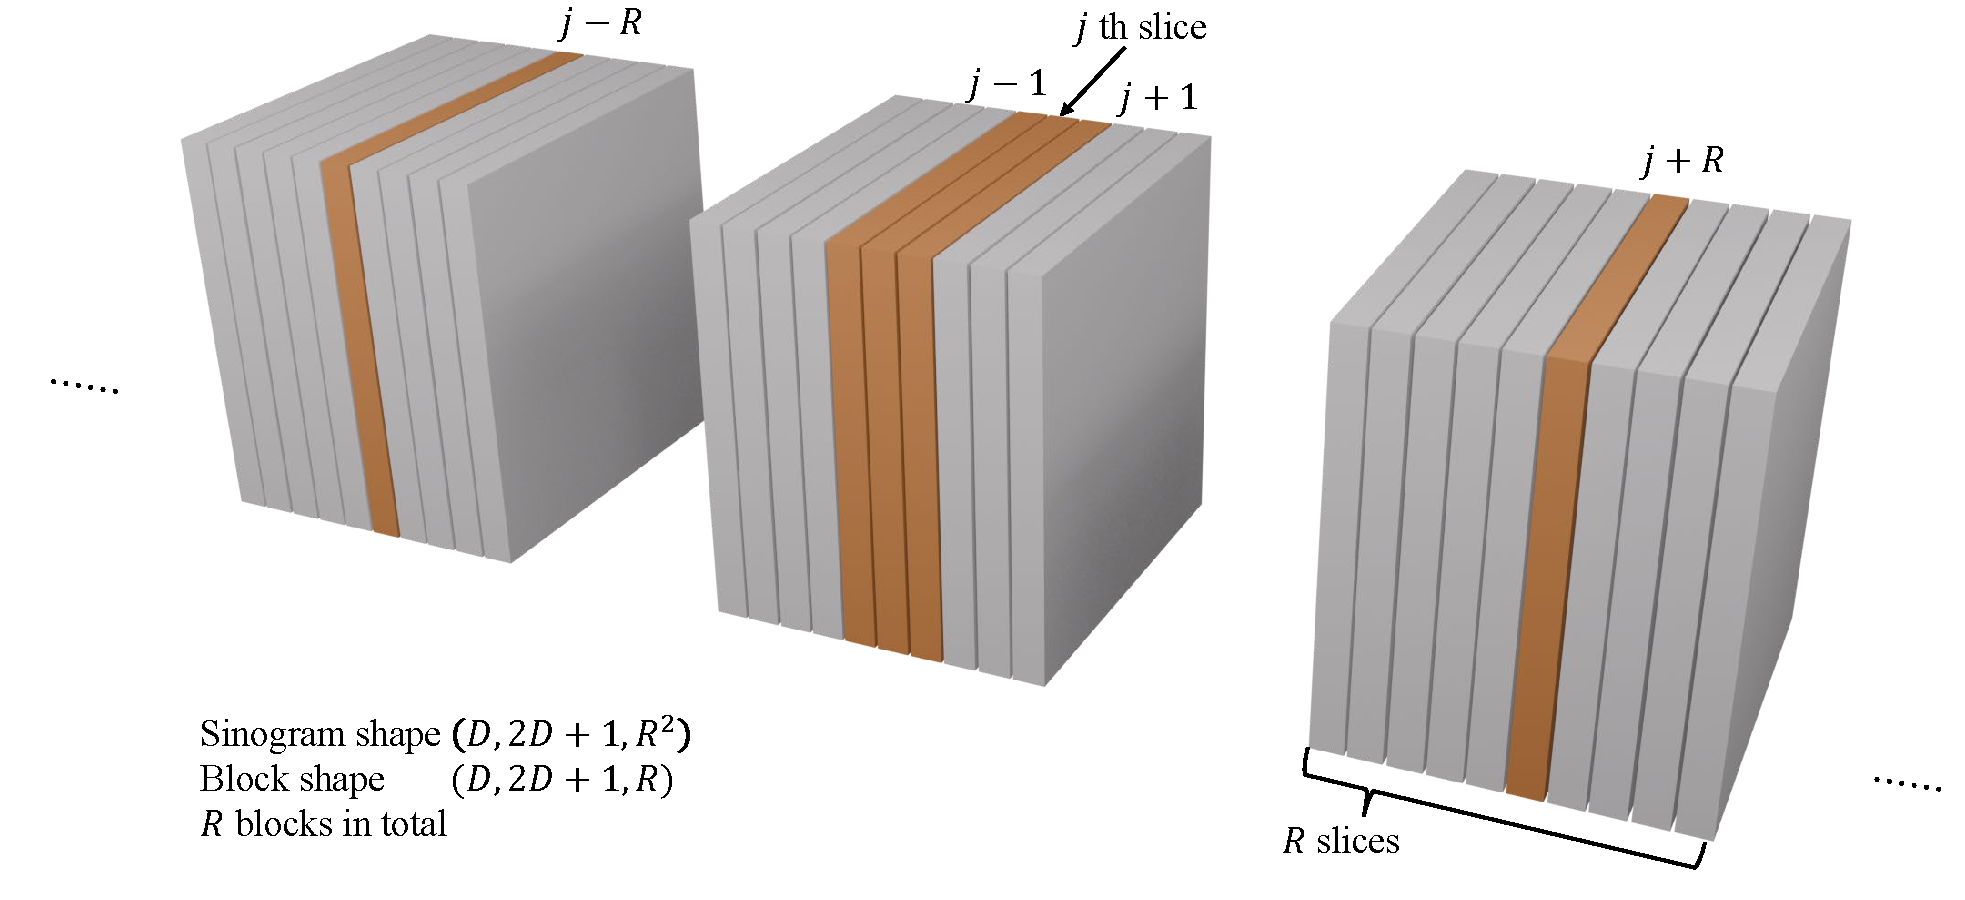
\includegraphics[width=0.96\textwidth]{Images/slices.pdf}
\vspace{-.3cm}
\caption{Visualization of the five-channel tensor preparation of sinogram data for training. Each cube represents a sinogram slice block with dimensions $(D, 2D+1, R^2)$. The orange highlighted parts are the selected slices ($j-R, j-1, j, j+1, j+R$), which form the five-channel input for the restoration model, showing the spatial and temporal relationships captured in each input tensor.}
\label{fig:sinogram_structure}
\end{figure*}



The model structure is shown in Tabel~\ref{tab:unet_architecture}.
Model training uses the Adam optimizer with an initial learning rate of $10^{-4}$ and adds   $10^{-5}$ weight decay to prevent overfitting. 
Training efficiency is enhanced through mixed precision computation and gradient scaling techniques, combined with a ReduceLROnPlateau dynamic learning rate scheduler (with a decay factor of 0.3 when validation loss shows no improvement for 3 consecutive epochs), achieving stable convergence.


\subsection{Image Refinement Based on U-Net and Diffusion Model}
\label{sec:diffusion_model}
Then, to further improve the image quality in geometry space, we have the second stage of our framework, which is a dual-model architecture that combines U-Net and diffusion model. The U-Net model is used to generate a coarse prediction of the image, while the diffusion model is used to refine the image by reconstructing the residual signal. This two-stage approach effectively balances reconstruction quality with computational efficiency.
Here we adopt almost the same architecture as that used in Ref. \cite{han2023} except some tweaks of the hyperparameters for the training
And they also use an auxiliary guidance strategy and a contrastive diffusion strategy to improve the reconstruction quality. The auxiliary guidance strategy uses neighboring axial slices and spectral information to provide additional context for the reconstruction, while the contrastive diffusion strategy ensures that the model produces anatomically plausible reconstructions specific to each individual scan. 
And we train the model using a combination of L1 loss and contrastive loss without pretrained weights. 

% \subsection{Evaluation Metrics}

% To comprehensively evaluate the performance of the reconstruction results of both sinogram and its reconstructed images, we use several quantitative metrics. These metrics measure the similarity between reconstructed images and ground truth images from different perspectives, including pixel-level accuracy, structural fidelity, and preservation of clinically relevant features.


% \textbf{Peak Signal-to-Noise Ratio (PSNR)} \cite{Hore2010PSNRvsSSIM} is a fundamental metric for evaluating reconstructed image quality. It is calculated based on Mean Squared Error (MSE) and usually expressed on a logarithmic scale. The definition of PSNR is:
% \begin{equation}
% \text{PSNR} = 10 \cdot \log_{10}\left(\frac{\text{MAX}_I^2}{\text{MSE}}\right),
% \end{equation}
% where $\text{MAX}_I$ represents the maximum possible pixel value of the image; for images normalized to the [0,1] range, $\text{MAX}_I = 1$. MSE is calculated as follows:
% \begin{equation}
% \text{MSE} = \frac{1}{mn}\sum_{i=0}^{m-1}\sum_{j=0}^{n-1}[I(i,j) - K(i,j)]^2,
% \end{equation}
% where $I$ and $K$ are the original and reconstructed images respectively, and $m$ and $n$ are the image dimensions. For three-dimensional PET image voxels, the MSE calculation extends to three dimensions.
% PSNR values are typically expressed in decibels (dB), with higher values indicating better reconstruction quality. In this study, PSNR values above 30dB typically indicate high-quality reconstruction.

% \textbf{Structural Similarity Index (SSIM)}: Although PSNR is intuitive, it cannot adequately reflect the human visual system's perception of structural information. SSIM addresses this deficiency by evaluating similarity in terms of brightness, contrast, and structure to more comprehensively assess image quality \cite{Wang2004SSIM}:
% \begin{equation}
% \text{SSIM}(x, y) = \frac{(2\mu_x\mu_y + c_1)(2\sigma_{xy} + c_2)}{(\mu_x^2 + \mu_y^2 + c_1)(\sigma_x^2 + \sigma_y^2 + c_2)},
% \end{equation}
% where $\mu_x$ and $\mu_y$ are the averages of images $x$ and $y$ respectively; $\sigma_x^2$ and $\sigma_y^2$ are their variances; $\sigma_{xy}$ is their covariance; and $c_1$ and $c_2$ are small constants set to avoid division by zero.
% SSIM values range between [-1,1], with 1 indicating that two images are identical. In medical image reconstruction, SSIM is particularly important because it better reflects the preservation of diagnostically relevant structures. 

% \textbf{Normalized Mean Square Error (NMSE)} normalizes the image error with respect to the energy of the original image \cite{Higashiyama2024NMSE}:
% \begin{equation}
% \text{NMSE} = \frac{\sum_{i,j,k}(X_{i,j,k} - \hat{X}_{i,j,k})^2}{\sum_{i,j,k}X_{i,j,k}^2},
% \end{equation}
% where $X$ and $\hat{X}$ are the original and reconstructed images respectively. A smaller NMSE indicates better reconstruction quality, and it is particularly useful for comparisons between different image sets and experimental setups as it eliminates the impact of image scale.




%!TEX root = ../Manual.tex
\section{Results}
\label{chap:results}
In order to investigate the effect of the form of loss on the reconstruction results while ensuring that the total amount of data loss remained constant, we varied the range of angles at which the data were missing and ensured that the total range of missing angles remained constant and repeated the experimental procedure. The results on test set are listed in Table~\ref{tab:results}. 
The table includes PSNR and SSIM values of the recovered sinogram data by the first stage Attention U-Net, the reconstruction from these sinogram, and the refined images from the reconstruction using the second stage model. The results indicate that our method achieves high-quality reconstruction performance, with PSNR values exceeding 30 dB and SSIM values above 0.95 for most cases. 

Figure~\ref{fig:pet_incomplete_reconstruction} shows the comparison between directly reconstructed results without any correction and the original image. As can be seen, due to incomplete sampling caused by data loss, there are significant differences between the directly reconstructed image and the original image. These phenomena indicate that traditional PET reconstruction methods face difficulties when applied to incomplete ring PET geometries, necessitating new methods to address the data loss problem.
\begin{table}[htbp]
    \centering
    \caption{Quantitative results for different angular-loss patterns}
    \label{tab:results}
    \begin{tabular}{ll ll}
    \hline \hline \addlinespace[2pt]
    \textbf{Lost angle range}&\textbf{Parameter} & \textbf{Mean}&\textbf{Std}\\
    \hline\addlinespace[2pt]
    \multirow{6}{*}{[30\degree, 90\degree] \& [210\degree, 270\degree]}
    &SSIM (refined)& 0.9902 &0.01232\\
    &PSNR (refined)& 35.36 dB&2.332 dB\\
    &SSIM& 0.9703 &0.01480\\
    &PSNR& 32.12 dB&2.650 dB\\
    &SSIM (sinogram)& 0.9827&0.001512\\
    &PSNR (sinogram)& 35.98 dB&0.3101 dB\\
    \hline
    \multirow{6}{*}{[60\degree, 120\degree] \& [240\degree, 300\degree]}
    &SSIM (refined)& 0.9924 &0.01302\\
    &PSNR (refined)& 34.97 dB&2.231 dB\\
    &SSIM& 0.9709&0.0134\\
    &PSNR& 32.91 dB&2.532 dB\\
    &SSIM (sinogram)& 0.9830&0.001612\\
    &PSNR (sinogram)& 35.91 dB&0.2713 dB\\
    \hline
    \multirow{6}{*}{\parbox{4.8cm}{[60\degree, 90\degree] \& [130\degree, 160\degree] \& [240\degree, 260\degree] \& [320\degree, 340\degree]}}
    &SSIM (refined)& 0.9958 &0.01152\\
    &PSNR (refined)& 35.92 dB&2.542 dB\\
    &SSIM& 0.9761&0.01315\\
    &PSNR& 33.10 dB&2.851 dB\\
    &SSIM (sinogram)& 0.9879&0.001349\\
    &PSNR (sinogram)& 38.41 dB&0.2629 dB\\
    \hline \hline
    \end{tabular}
\end{table}
Figure~\ref{fig:pet_reconstruction_results} demonstrates the model's capability in reconstructing incomplete sinograms. After 40 rounds of training, the model can effectively recover complete sinogram structures from inputs with missing angular data. From the figure, it can be observed that although the input sinogram (left) has large-scale data loss, the model's predicted sinogram (middle) successfully restores a structure and signal distribution highly similar to the real sinogram (right). This indicates that our proposed two-stage restoration framework can effectively learn the potential structures and features in sinograms, enabling accurate reconstruction even in cases of severe data loss.
\begin{figure*}[ht]
    \centering
    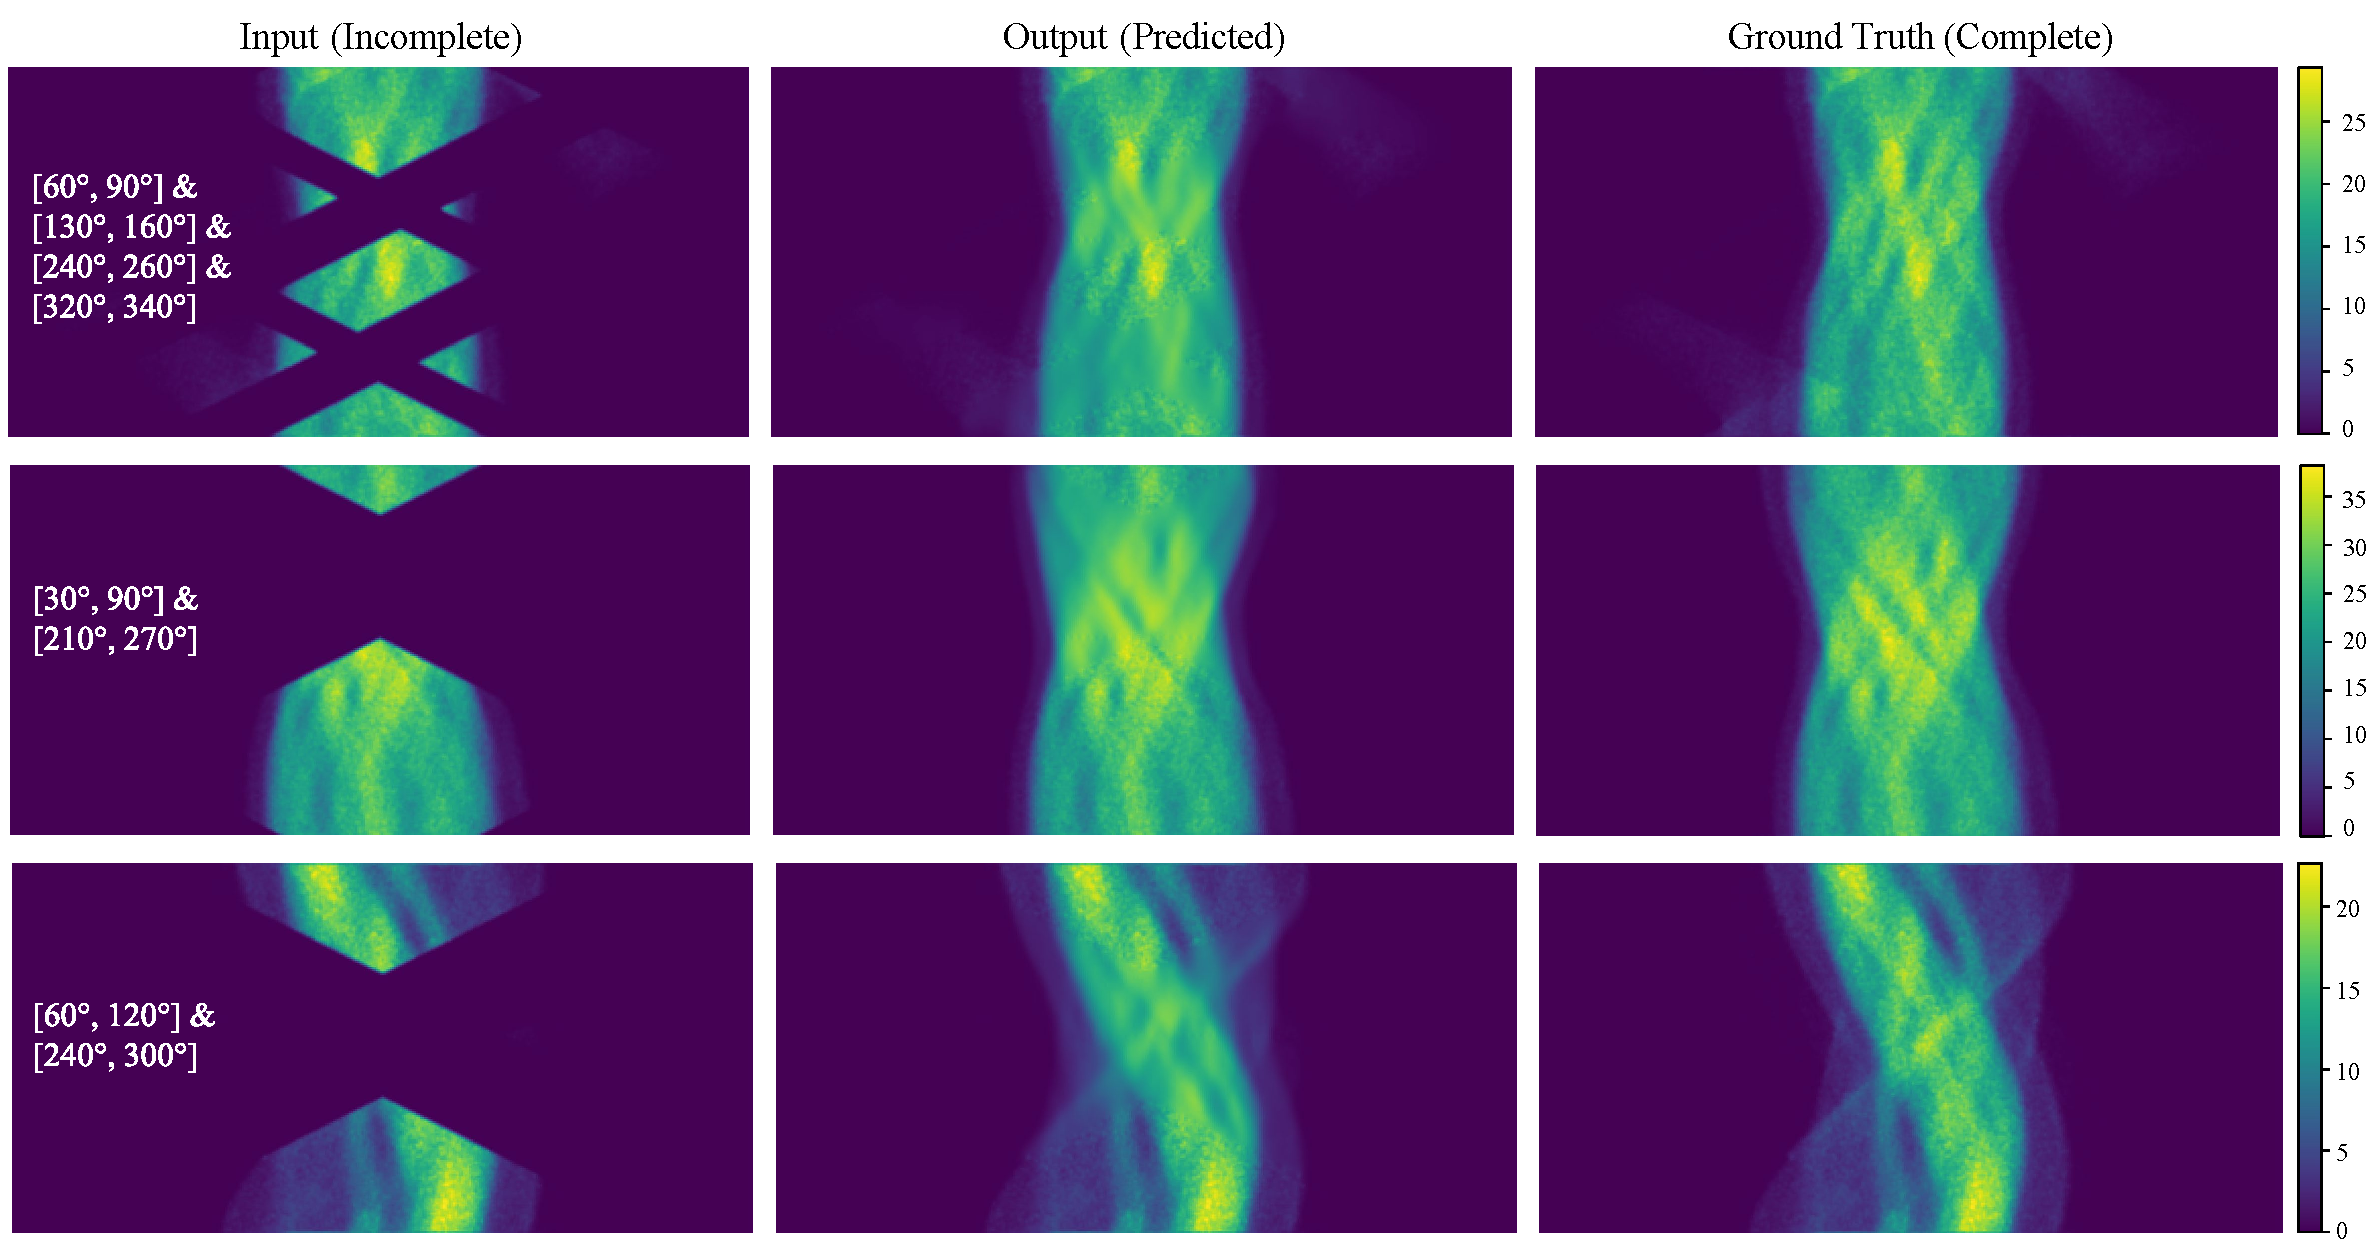
\includegraphics[width=\textwidth]{Images/sinograms.pdf}
    \vspace{-1cm}
    \caption{Comparison of PET sinogram reconstruction results after training (metrics are shown in Tabel~\ref{tab:results}). Each row displays three images: the left shows the incomplete input sinogram with missing angular data, the middle shows the model-predicted complete sinogram, and the right shows the complete real sinogram. And each row corresponds to a different angular loss range, as indicated in the first column. }
    \label{fig:pet_reconstruction_results}
\end{figure*}
Figure~\ref{fig:pet_brain_reconstruction} shows the PET image quality generated from the reconstructed sinogram. Its PSNR reached 35.92 dB and SSIM was 0.9958. By comparing the original PET brain image (left) with the reconstructed PET image (right), it can be seen that the reconstructed image successfully preserves key anatomical structures and tracer distribution features from the original image. Particularly in the cerebral cortex and basal ganglia regions, the reconstructed image clearly preserves the boundaries and contrast of high uptake areas. 

\begin{figure}[ht]
    \centering
    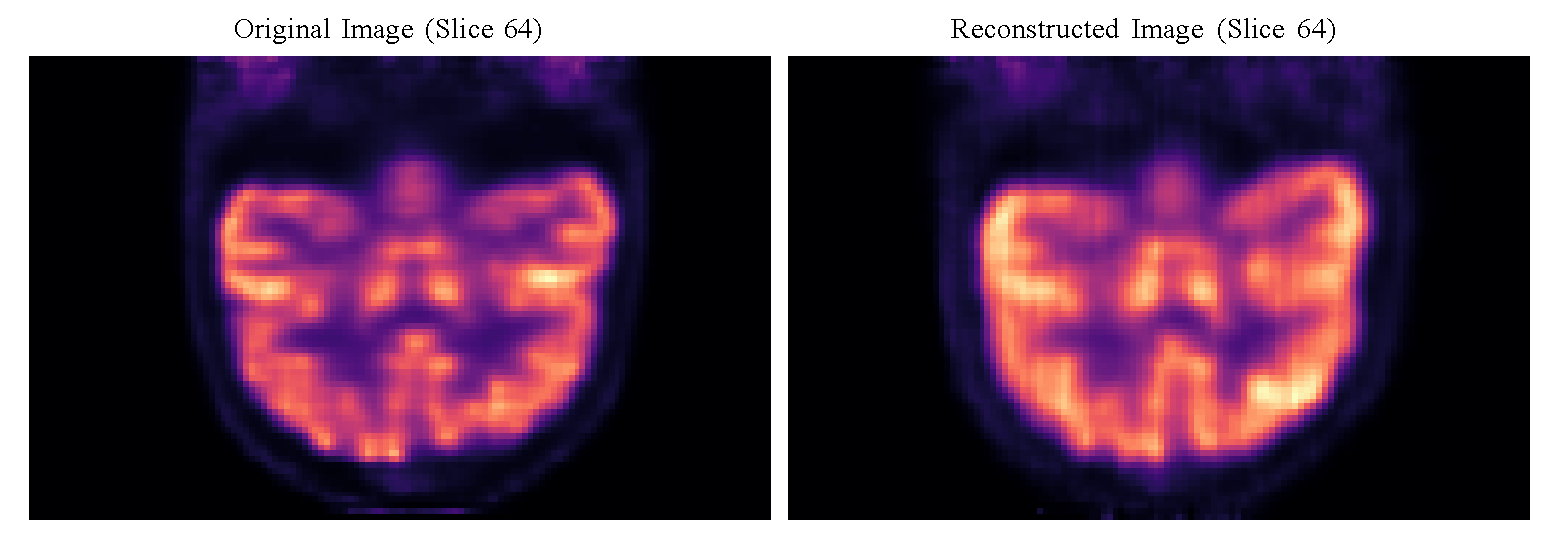
\includegraphics[width=\textwidth]{Images/compare_reconstruction_restoration2}
    \vspace{-1cm}
    \caption{Comparison of original PET brain image (left) with PET image reconstructed from predicted sinogram (right), both showing the 64th layer slice with SSIM of 0.9703 and PSNR of 32.12 dB. The lost angle range is [30\degree, 90\degree] and [210\degree, 270\degree]. 
    }
    \label{fig:pet_brain_reconstruction}
\end{figure}


\section{Conclusion and Discussion}
\label{chap:conclusion}

\begin{figure}[ht]
    \centering
    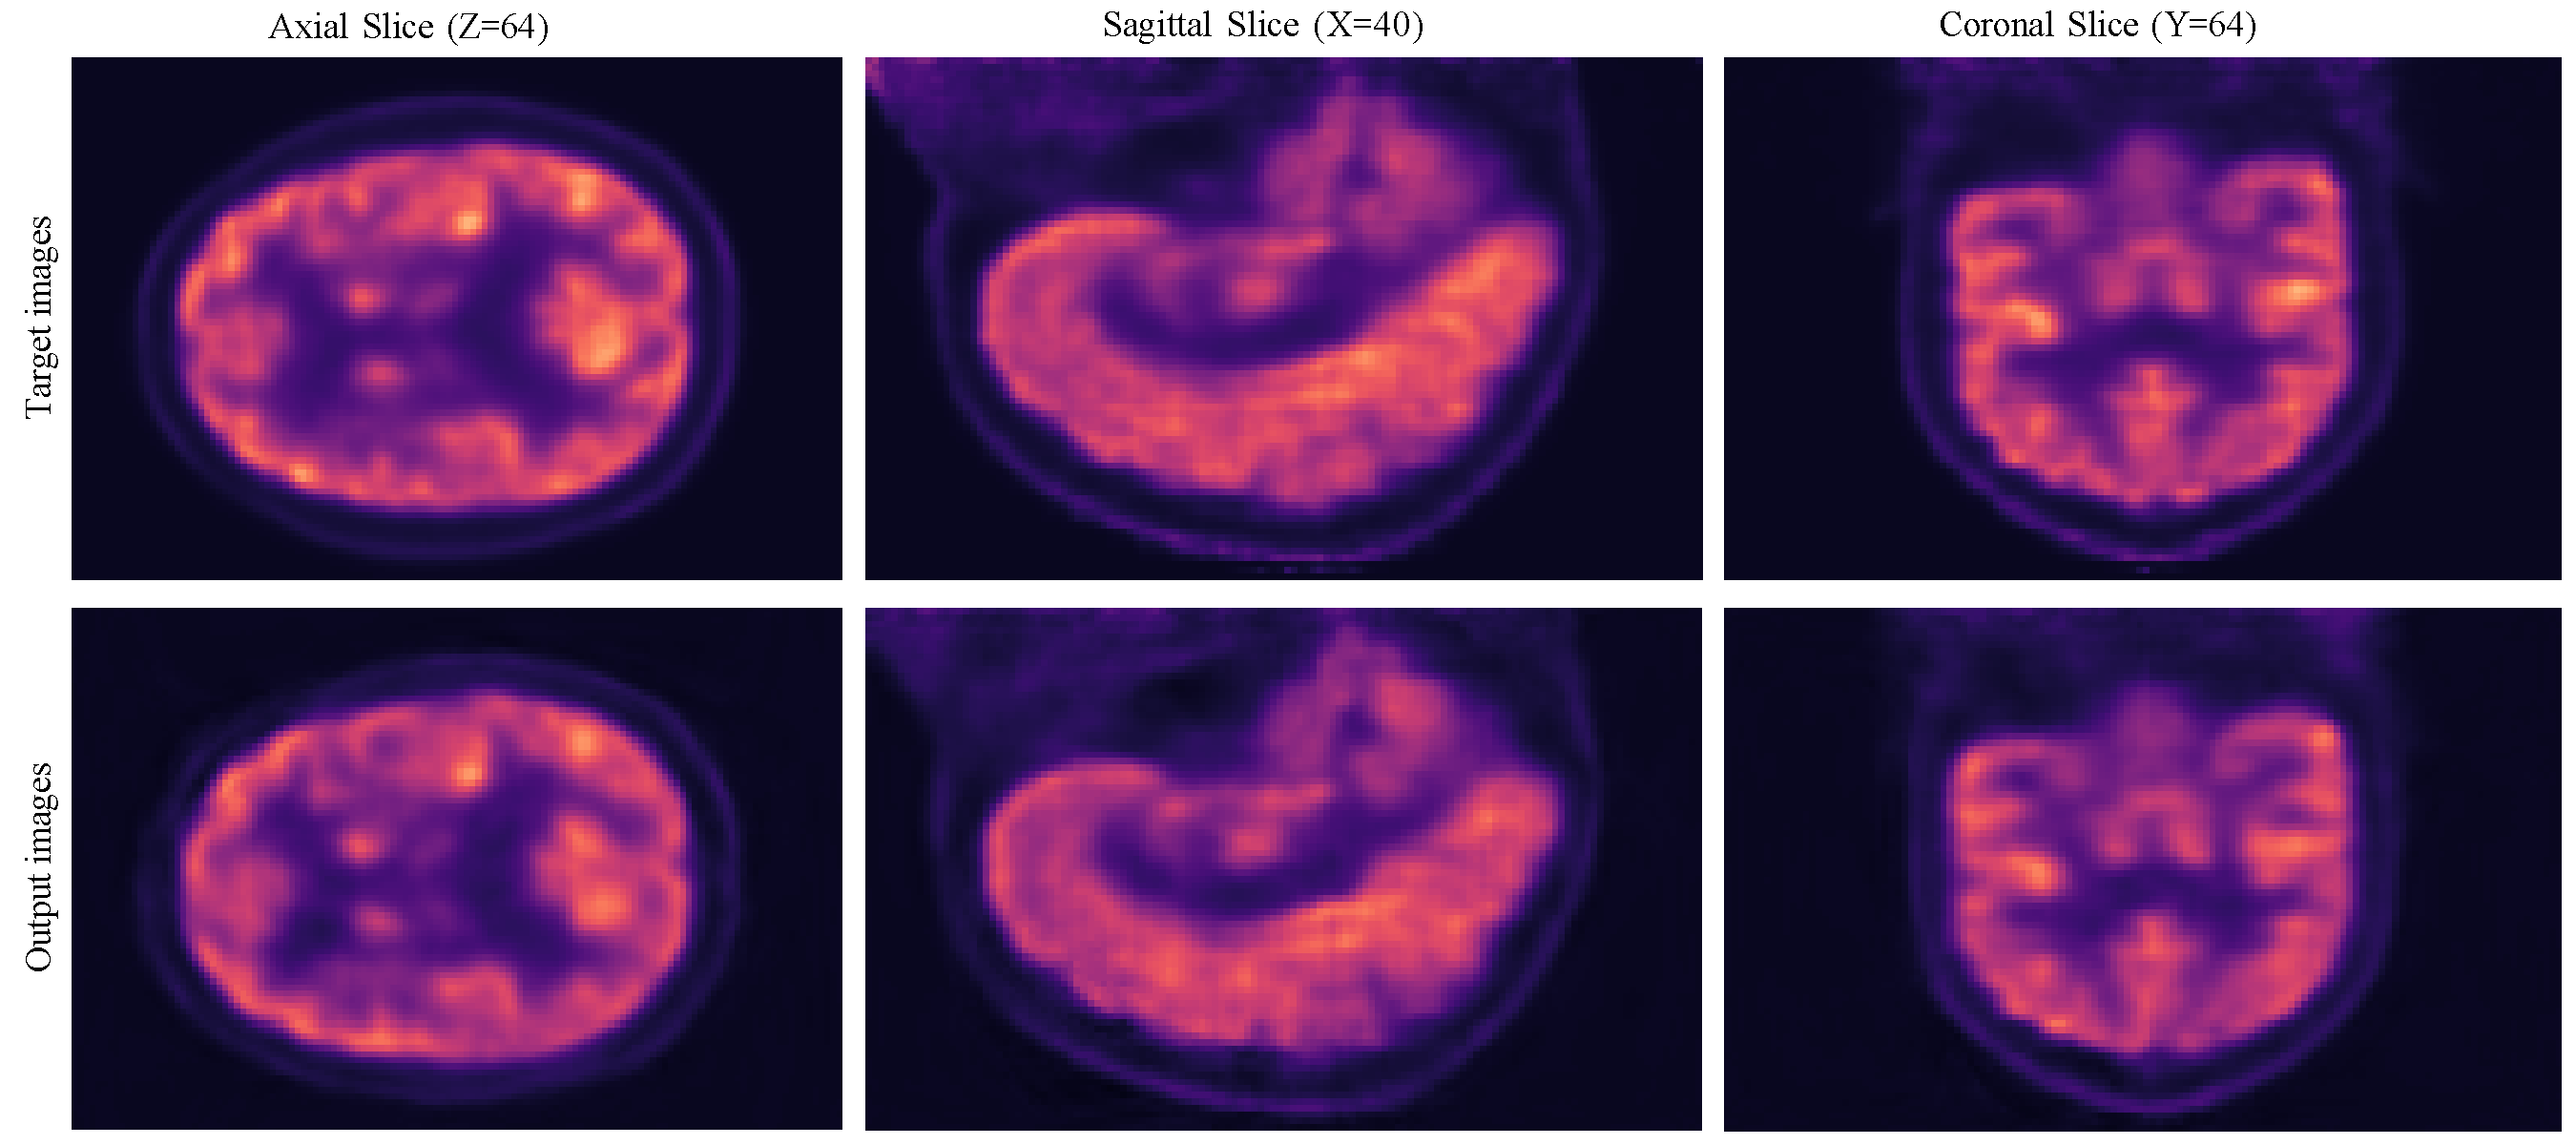
\includegraphics[width=\textwidth]{Images/target_outputs.pdf}
    \vspace{-1cm}
    \caption{Comparison of original PET brain image (top) with PET image refined from the raw images reconstructed from predicted sinogram (bottom) with the SSIM of 0.9902 and PSNR of 35.36 dB. The lost angle range is [30\degree, 90\degree] and [210\degree, 270\degree]. The axial slices should be $128\times128$, but we only show the central $128\times80$ part. 
    }
    \label{fig:compare_reconstruction_restoration}
\end{figure}

From the experimental results, we can  confirm that our two-stage reconstruction can effectively recover  PET images from incomplete ring geometries. And we also have several important findings. 
First, our model performs remarkably well despite operating with approximately 50\% missing data and $1/3$ missing detectors, in which case direct reconstruction without restoration will cause a chaos. 
But our approach was still able to achieve PSNR values above 30 dB and SSIM scores above 0.97 for images, indicating successful ability to recover missing information of key structural features.

While the total amount of missing data remains constant, the specific distribution of the missing affects the quality of the recovery. The model extrapolates the missing parts with the help of existing data, and when the sinogram contains an entire missing region, the model will infer the missing parts from farther away, which will lead to a decrease in the quality of recovery, as shown in the second and third rows of Figure~\ref{fig:pet_reconstruction_results}. However, when the missing and intact parts are interleaved, the quality of recovery improves because the model is able to extrapolate from a closer and thus more accurate location. 

Additionally, we also found that attention mechanism is essential for the model to learn the relationship between different parts of the sinogram regardless of distances between them.
Comparing the second and third rows of Figure~\ref{fig:pet_reconstruction_results}, we can observe different patterns of missing data. In the third row, the missing portions are primarily concentrated in the middle region of the sinogram, with relatively balanced data preserved in both the upper and lower sections. In contrast, the second row's missing data extends closer to the upper part of the sinogram, with only a narrow band of preserved data in the upper region.  
So if the model can only capture short distance relationships, obviously the second row will be more difficult to recover than the third row because the model has to extrapolate the missing parts from farther away.
However, the results from Table~\ref{tab:results} show that the PSNR and SSIM of the second row are actually quite similar to those of the third row. This indicates that the attention mechanism can help the model learn the relationship between different parts of the sinogram regardless of distances between them, which is very important for the model to leverage the existing data effectively to recover the missing parts.

Our dataset with only adjacent slices can solve the memory usage problem when processing super-large sinogram tensors in a simple way. Instead of processing the whole tensor of the size $(182, 365, 1764)$ all as a time, we divided it into $R\times(D, 2D+1, R)$ tensors and process them sequentially. But we will lose the context for each slice. And by inputing five input channels per slice (the current slice, two spatial neighbors, and two temporal neighbors), we created a contextually sufficient representation and also lower memory costs. This approach  avoid memory limitations and also enhance reconstruction quality by considering correlated information from adjacent slices, showing an average increase of 1.24dB in PSNR and 0.052 in SSIM compared to single-slice processing.

For more robust evaluation and enough data for the second stage, we used 6-fold cross-validation on our 206 volumes dataset. 
This validation strategy minimizes the influence of random variation and provides more reliable performance metrics. The cross-validated results confirmed this performance advantages with PSNR of 35.6421 dB and SSIM of 0.9958 on the validation set. 
On the contrary, if we do not use cross validation, we can only use the data on the test set (about 36 images) for both training and testing on the model of the second stage. Because of the data leakage, the prediction on the training set cannot be used for the second stage model 

Although more complex generative models like diffusion models and GANs have been used in low-dose PET reconstruction and denoising and also shown their strong capabilities in those tasks, our approach also achieves excellent results with more computationally efficient models. This is really important in clinical applications, where timely image production is essential.
The SSIM values in final reconstructed images is slightly lower compared to restored sinograms, which means that some information is lost in the OSEM reconstruction. 
Therefore, our sinogram restoration performance is actually better than what the final image metrics show, because the OSEM reconstruction of both complete sinogram and predicted sinogram introduces their approximations, making final metrics slightly worse.




% However, we still have some limitations in this study: although we adopted 2D slice processing (enhanced by adjacent slices) to improve memory efficiency, a fully 3D version might perform better as it has a more comprehensive context of sinogram. Or we can also try to use recurrent neural network or attention mechanism to capture more precise relationships between difference slices. 
% Additionally, we are mainly validating for ring-type and partial angular coverage, but missing detectors in real-world situation might lead to more complex missing patterns, requiring more advanced geometric modeling methods.
However, our study has several important limitations that should be acknowledged. First, our simulation employed idealized detection settings with uniform detector properties, which significantly differs from real-world PET systems where individual detectors exhibit variations in sensitivity, energy resolution, and timing characteristics. This idealization may limit the direct applicability of our method to clinical scanners. Second, we validated our approach exclusively on brain PET data from a limited cohort, without exploring its generalization to other anatomical regions or pathological conditions. The method's performance on whole-body PET or in the presence of lesions remains untested. Third, while we adopted 2D slice processing enhanced by adjacent slices to improve memory efficiency, this approach may miss important 3D contextual information that could be leveraged by fully volumetric processing. 
% Fourth, our simulation framework, though effective for this proof-of-concept study, lacks the validation and widespread acceptance of established tools like GATE, potentially limiting the reproducibility and clinical relevance of our findings. 
Finally, the specific scanner geometry used (253.71 mm radius) represents only one configuration, and the model's adaptability to different scanner dimensions and detector arrangements requires further investigation.



% Looking toward future improvements, positional encoding could also be incorporated to better account for the sequential nature of axial slices. Additionally, while we tested transformer-based architectures like UNETR and TransUNet, they were slightly outperformed by Attention U-Net in our specific task. 
% Therefore, for our current dataset size, convolutional architectures remains beneficial. However, if we can have larger datasets, transformer-based approaches might fulfil their full potential.

Looking toward future improvements, several directions warrant exploration. Validation with experimental data from real PET scanners, including systems with known detector failures or irregularities, would be essential for clinical translation. Extension to diverse anatomical regions and pathological conditions would demonstrate the method's broader applicability.
% Integration with validated simulation frameworks like GATE would enhance the reliability and acceptance of our results. 
To better capture inter-slice relationships while maintaining computational efficiency, hybrid approaches combining recurrent neural networks or transformer-based attention mechanisms with our current architecture could be explored. Additionally, incorporating physics-based constraints and detector-specific modeling could help bridge the gap between idealized simulations and real-world complexities. While transformer-based architectures like UNETR and TransUNet were slightly outperformed by Attention U-Net in our current study, larger and more diverse datasets might unlock their full potential for this reconstruction task.



%!TEX root = ../Manual.tex
\section{Acknowledgments}
I would like to express my sincere gratitude to senior students, Xiaoyu Chen for insightful discussions and suggestions.
The conclusions and analyses presented in this publication were produced using the following software: Python (Guido van Rossum 1986) \cite{10.5555/1593511}, Opencv (Intel, Willow Garage, Itseez) \cite{itseez2015opencv}, Scipy (Jones et al. 2001) \cite{2020SciPy-NMeth}, PyTorch  (Meta AI September 2016) \cite{NEURIPS2019_9015}, Matplotlib (Hunter 2007) \cite{Hunter:2007} and Seaborn \cite{Waskom2021}.
The dataset for this study can be found in \url{https://github.com/Show-han/PET-Reconstruction.git}.
% \appendix

% \section{Parameters of models}
% \label{sec:appendix}

% The parameters of the five-channel U-Net network structure are shown in Table~\ref{tab:unet_architecture}. We also have skip connections between the encoder and decoder blocks, which are not shown in the table. 

% \begin{table}[htbp]
%     \centering
%     \caption{Five-channel Attention U-Net backbone}
%     \vspace{0.1cm}
%     \label{tab:unet_architecture}
%     \begin{tabular}{@{}l c c@{}}
%         \toprule
%         \textbf{Stage / block(s)} & \textbf{Main ops (per level)} & \textbf{$C_\text{out}$} \\
%         \midrule
%         Input & --- & 5 \\[3pt]
        
%         \multirow{2}{*}{Encoder $\times$4} 
%           & [Conv $3\times3$ + BN + ReLU]$\times2$ & \multirow{2}{*}{64, 128, 256, 512}\\
%           & MaxPool $2\times2$                        & \\[3pt]
        
%         Bottleneck & [Conv $3\times3$ + BN + ReLU]$\times2$ & 1024 \\[3pt]
        
%         \multirow{2}{*}{Decoder $\times$4}
%           & Upsample ($\uparrow$2) + skip concat      & \multirow{2}{*}{512, 256, 128, 64}\\
%           & [Conv $3\times3$ + BN + ReLU]$\times2$  & \\[3pt]
        
%         Output & Conv $1\times1$ & 5 \\
%         \bottomrule
%         \end{tabular}
        
%   \end{table}
  

% All hyperparameters required to replicate the run are collected in Table~\ref{tab:num-hparams}.

% \begin{table*}[htbp]
%   \centering
%   \label{tab:num-hparams}
  
%   \caption{Numerical hyper-parameters for the stage-2 run}
%   \vspace{0.1cm}
%   % ---------- first half ----------
%   \begin{minipage}[t]{0.4\linewidth}\centering
%     \begin{tabular}{@{}l r@{}}
%       \toprule
%       \textbf{Hyper-parameter} & \textbf{Value}\\
%       \midrule
%       \multicolumn{2}{@{}l}{\emph{Data}}\\
%       \quad batch\_size & 12\\
%       \quad l\_resolution (=r) & 64\\[2pt]
%       \multicolumn{2}{@{}l}{\emph{U-Net}}\\
%       \quad in\_channel & 1\\
%       \quad out\_channel & 1\\
%       \quad inner\_channel & 64\\
%       \quad res\_blocks & 3\\[2pt]
%       \multicolumn{2}{@{}l}{\emph{diffusion model}}\\
%       \quad in\_channel & 2\\
%       \quad out\_channel & 1\\
%       \quad inner\_channel & 32\\
%       \quad res\_blocks & 3\\
%       \bottomrule
%     \end{tabular}
%   \end{minipage}%
%   % ---------- second half ----------
%   \begin{minipage}[t]{0.4\linewidth}\centering
%     \begin{tabular}{@{}l r@{}}
%       \toprule
%       \textbf{Hyper-parameter} & \textbf{Value}\\
%       \midrule
%       \multicolumn{2}{@{}l}{\emph{Channel multipliers}}\\
%       \quad levels & 1, 2, 3, 4\\[2pt]
%       \multicolumn{2}{@{}l}{\emph{Diffusion process}}\\
%       \quad image\_size & 128\\
%       \quad $T_{\text{train}}$ & 2 000\\
%       \quad $T_{\text{val}}$ & 10\\
%       \quad $\beta_{\mathrm{start}}$ & $1\times10^{-6}$\\
%       \quad $\beta_{\mathrm{end,train}}$ & 0.01\\
%       \quad $\beta_{\mathrm{end,val}}$ & 0.5\\[2pt]
%       \multicolumn{2}{@{}l}{\emph{Optimisation}}\\
%       \quad n\_iter & 600 000\\
%       \quad learning rate & 0.0002\\
%       \quad EMA decay & 0.9999\\
%       \bottomrule
%     \end{tabular}
%   \end{minipage}
% \end{table*}




% \section*{References}

% \nocite{*}
\bibliographystyle{unsrt}
\bibliography{sinogram}




\end{document}
